% What do i want to share 
% the temperature model used 
% how I calculated the constants 
% How I will be varying the coolant channel shape 

\section{Moltres AHTR Steady-State Temperature Model}
One of the ROLLO AHTR optimization objectives is minimizing the maximum 
temperature in the slab. 
A neutronics simulation cannot calculate maximum temperature; thus, I introduced 
AHTR slab temperature modeling with Moltres.
I used OpenMC to generate multigroup neutronics data for the AHTR slab at 948K 
for four energy groups and eight precursor groups based on the following 
spatial and energy homogenization. 

For spatial homogenization of the straightened \gls{AHTR} fuel slab, I used 
OpenMC's \textit{cell} domain type to compute multigroup cross sections for 
different \textit{cells}. 
I discretized the slab into 13 \textit{cells}: FLiBe, left graphite, right 
graphite, and ten fuel cells (each cell has a different packing fraction). 
Figure \ref{fig:straightened_slab_mg} illustrates the \gls{AHTR} spatial 
homogenization for the OpenMC multigroup calculation. 
\begin{figure}[H]
    \centering
    
\includegraphics[width=\linewidth]{straightened_slab_mg.png}
    \raggedright
    \resizebox{0.5\textwidth}{!}{
        \hspace{1cm}
        \fbox{\begin{tabular}{llll}
            \textcolor{fhrblue}{$\blacksquare$} & FLiBe & 
            \textcolor{fhrgrey}{$\blacksquare$} & Left Graphite \\
            \textcolor{fhrred}{$\blacksquare$} & Right Graphite &
            \textcolor{fhrpink}{$\blacksquare$} & Fuel cell 1 $\&$ 6 \\
            \textcolor{fhryellow}{$\blacksquare$} & Fuel cell 2 $\&$ 7 &
            \textcolor{fhrorange}{$\blacksquare$} & Fuel cell 3 $\&$ 8 \\
            \textcolor{fhrgreen}{$\blacksquare$} & Fuel cell 4 $\&$ 9 &
            \textcolor{fhrpurple}{$\blacksquare$} & Fuel cell 5 $\&$ 10 \\
            \end{tabular}}}
    \caption{Straightened \acrfull{AHTR} fuel slab spatially discretized into 
    13 \textit{cells} for OpenMC multigroup calculation.}
    \label{fig:straightened_slab_mg}
\end{figure}
I used the four group energy structure derived by Gentry et al. 
\cite{gentry_development_2016} for \gls{AHTR} geometries. 
Table \ref{tab:energy_structures} defines the group boundaries. 
\begin{table}[H]
    \centering
    \onehalfspacing
    \caption{4-group energy structures for \acrfull{AHTR} geometry 
    derived by \cite{gentry_development_2016}.}
	\label{tab:energy_structures}
    \footnotesize
    \begin{tabular}{lll}
    \hline
    \multicolumn{3}{c}{\textbf{Group Boundaries [MeV]}} \\ 
    \hline
    \textbf{Group $\#$}& \textbf{Upper Bound} & \textbf{Lower Bound}  \\
    \hline 
    1 & $2.0000\times 10^1$ & $9.1188\times 10^{-3}$ \\ 
    2 & $9.1188\times 10^{-3}$ & $2.9023\times 10^{-5}$\\
    3 & $2.9023\times 10^{-5}$ & $1.8554\times 10^{-6}$\\
    4 & $1.8554\times 10^{-6}$ & $1.0000\times 10^{-12}$\\
    \hline
    \end{tabular}
\end{table}

The Moltres AHTR Steady-State Temperature Model is a 2D model of the AHTR slab's 
x-y cross-section with Figure \ref{fig:straightened_slab_mg}'s geometry. 
% 3d model with unit thickness 
The model first solves the slab's neutronics and uses that to solve the slab's 
temperature distribution for a defined power.
The temperature model assumes conductive heat transfer throughout the domain 
and heat removal by uniform salt flow in the coolant region. 
These assumptions ignore turbulent effects that would most likely be present. 
However, an in-depth AHTR Moltres model that includes turbulence modeling is 
out of scope for this dissertation. 

Equation \ref{eq:moltres-temp} describes Moltres' governing equation for temperature
\begin{align}
    \label{eq:moltres-temp}
    \rho c_p\frac{\partial T}{\partial t} &+ \nabla\cdot\left(\rho
        c_f \vec{u}\cdot T -k\nabla T\right) =  Q
\end{align} 
In the 2D cross-sectional AHTR Steady-State Temperature Model, I ignore the 
time-dependent and velocity-dependent terms since I am solving for steady-state 
and there is no moving fuel: 
\begin{align}
    - \nabla \cdot (k_i \nabla T) &= Q_i
\intertext{where:}
k_i &= \mbox{thermal conductivity of material i} \nonumber \\
T &= \mbox{temperature in the slab} \nonumber \\
Q_i &= \mbox{source or sink term in material i} \nonumber
\end{align} 
Equation \ref{eq:moltres-source-term} defines the fuel cells' fission source term.
\begin{align}
    \label{eq:moltres-source-term}
        Q_f &= \sum_{g=1}^G \epsilon_{f,g}\Sigma_{f,g}\phi_g
    \intertext{where} 
    Q_f &= \mbox{source term } [\frac{MeV}{cm^3s}] \nonumber \\
    G &= \mbox{number of discrete neutron energy groups, g } [-] \nonumber \\
    \epsilon_{f,g} &= \mbox{heat produced per fission from neutrons in group g} [MeV] \nonumber \\
    \Sigma_{f,g} &= \mbox{macroscopic cross section for fission due to neutrons in group g } [\frac{1}{cm}] \nonumber \\
    \phi_g &= \mbox{flux of neutrons in group g } [\frac{n}{cm^2s}]\nonumber
    \end{align}
The heat removal from the AHTR fuel slab:
\begin{align}
    Q &= h \cdot A \cdot(T(\vec{r})-T_{ref})
\intertext{where:}
Q &= \mbox{heat removal rate for 1cm thin slice of AHTR slab [W/cm]} \nonumber \\
h &= \mbox{heat transfer coefficient } [\frac{W}{cm^3 \cdot K}] \nonumber \\
A &= \mbox{coolant area } [cm^2] \nonumber \\
T(\vec{r}) &= \mbox{temperature at point $\vec{r}$ [K]} \nonumber \\
T_{ref} &= \mbox{reference temperature [K]} \nonumber
\end{align}
Table \ref{tab:heat-exchanger-constants} shows reference temperature and heat 
transfer coefficient values for the convective heat transfer process.
\begin{table}[H]
    \centering
    \onehalfspacing
    \caption{AHTR Fuel Slab's heat transfer constants.}
	\label{tab:heat-exchanger-constants}
    \footnotesize
    \begin{tabular}{llll}
    \hline 
    \textbf{Constant}& \textbf{Value}& \textbf{Units} & \textbf{Notes} \\
    \hline 
    h & 990 & $\frac{W}{cm \cdot K}$ & Calculated in Eq. \ref{eq:calc-htc} \\
    $T_{ref}$ & 923 & K & AHTR Inlet Temperature \\ %cite ahtr 923K inlet temp 
    \hline
    \end{tabular}
\end{table} 
I calculated the heat transfer coefficient ($h$) using Equation \ref{eq:calc-htc}
with the following assumptions: 
\begin{itemize}
    \item slab generates a constant amount of power, all of which is removed 
    by the coolant
    \item linear increase in temperature from inlet to outlet 
\end{itemize} 
\begin{align}
    \label{eq:calc-htc}
    h &= \frac{P_{dz}}{V_{coolant}} \div \Delta T \\
      &= \frac{1456 W/cm}{23.1cm \times 0.35cm \times 1cm \times 2} \div 0.0909 K/cm \nonumber \\
      &= 990 W cm^{-3}K^{-1} \nonumber 
\intertext{and}
\Delta T  &= \frac{T_{total}}{H} = \frac{50 K}{550 cm} = 0.0909 K/cm
\intertext{where:}
h &= \mbox{heat transfer coefficient } [\frac{W}{cm^3 \cdot K}] \nonumber \\
P_{dz} &= \mbox{power produced in 1cm AHTR slab $\Delta z$ slice [$W/cm$]}\nonumber \\
V_{coolant} &= \mbox{coolant volume in AHTR slab [$cm^3$]} \nonumber \\
\Delta T &= \mbox{temperature change across 1cm AHTR slab $\Delta z$ slice [$K$]}\\
T_{total} &= \mbox{total temperature change from inlet to outlet [$K$]} \nonumber \\
H &= \mbox{AHTR height from inlet to outlet [cm]} \nonumber 
\end{align}

Figure \ref{fig:ahtr_constant_temp} shows the Moltres-generated temperature 
distribution with an average and maximum temperature of 1019K and 1128K, 
respectively.
\begin{figure}[H]
    \centering
    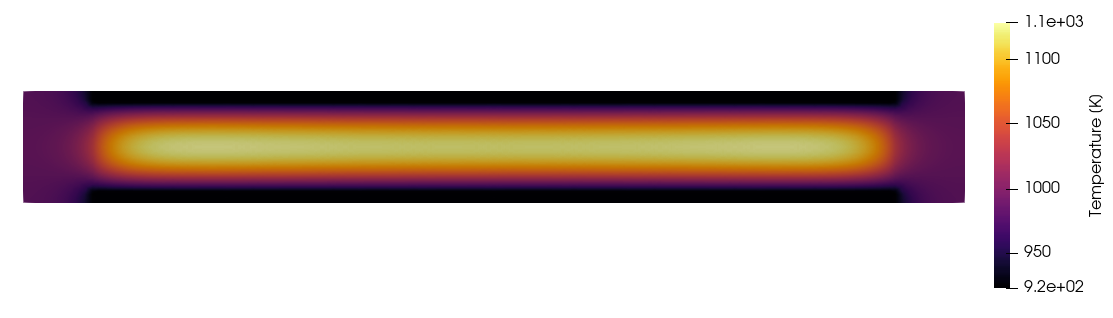
\includegraphics[width=\linewidth]{ahtr_constant_temp.png}
    \caption{AHTR fuel slab's Moltres generated temperature distribution for a 
    slab with a constant packing fraction of 0.0979 across ten fuel cells.}  
    \label{fig:ahtr_constant_temp}
\end{figure}
The temperature distribution is consistent with previous temperature models of 
the AHTR fuel slabs that report an average fuel kernel temperature of 1125K 
\cite{ramey_methodology_2021}. 
Model differences include that Ramey \cite{ramey_methodology_2021} utilized a 
1D temperature model with the original 4-layer TRISO model from the FHR benchmark. 
This model is 2D and randomly disperses TRISO particles throughout the 
slab while keeping the same overall packing fraction as the FHR benchmark. 

\pagebreak

\section{FliBE Coolant Channel Shape Variation}
In the ROLLO optimization simulations, I vary the FliBE coolant channel shape 
while holding the total coolant volume constant.  
Figure \ref{fig:ahtr-coolant-shape-variation-3} shows an example of how I will 
vary the coolant channel's shape. 
I model the variation in coolant channel shape with a sinusoidal-like pattern, 
using OpenMC's cylinder surfaces.
Varying the radius of the cylinder results in the depth and frequency of the coolant 
channel shape minimicing a sinusoidal pattern.
I calculated the heat transfer coefficient for the Moltres AHTR temperature model 
(Equation \ref{eq:calc-htc}) with the assumption that the slab generates a 
constant amount of power and coolant removes all the heat.
Since the coolant volume is held constant through the coolant channel 
optimization process, I use the same heat transfer coefficient ($h$)
for all the AHTR Moltres temperature models of varying coolant channel shapes.   
\begin{figure}[H]
    \centering
    \begin{subfigure}{\textwidth}
        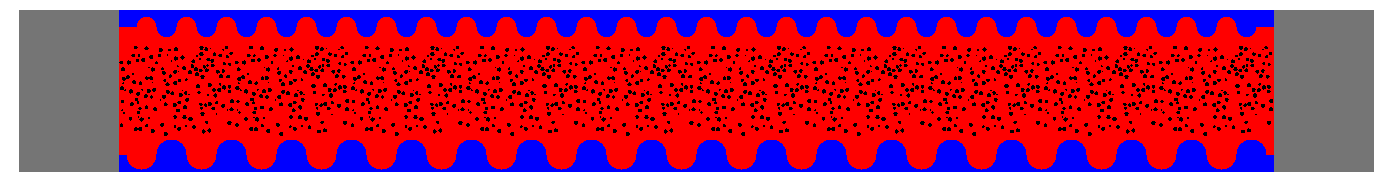
\includegraphics[width=\linewidth]{ahtr-coolant-shape-variation-3.png}
        \caption{Example of the coolant shape variation.}
        \label{fig:ahtr-coolant-shape-variation-3}
    \end{subfigure}
    \caption{AHTR Coolant Shape Variation}  
    \label{fig:ahtr-coolant-shape-variation}
\end{figure}